
%% LLT: Turn off some annoying warnings...
\RequirePackage{silence}
\WarningFilter{titlesec}{Non standard sectioning command}
\WarningFilter{scrreprt}{Usage of package}
\WarningFilter{scrreprt}{Activating an ugly workaround}

% **************************************************
% Document Class Definition
% **************************************************
\documentclass[%
	paper=A4,					% paper size --> A4 is default in Germany
	twoside=true,				% onesite or twoside printing
	openright,					% doublepage cleaning ends up right side
	parskip=full,				% spacing value / method for paragraphs
	chapterprefix=true,			% prefix for chapter marks
	11pt,						% font size
	headings=normal,			% size of headings
	bibliography=totoc,			% include bib in toc
	listof=totoc,				% include listof entries in toc
	titlepage=on,				% own page for each title page
	captions=tableabove,		% display table captions above the float env
	draft=false,				% value for draft version
]{scrreprt}%

% **************************************************
% Debug LaTeX Information
% **************************************************
%\listfiles

% **************************************************
% Information and Commands for Reuse
% **************************************************
\newcommand{\thesisTitle}{The Clean Thesis Style}
\newcommand{\thesisName}{Ricardo Langner}
\newcommand{\thesisSubject}{Documentation}
\newcommand{\thesisDate}{August 26, 2015}
\newcommand{\thesisVersion}{My First Draft}

\newcommand{\thesisFirstReviewer}{Jane Doe}
\newcommand{\thesisFirstReviewerUniversity}{\protect{Clean Thesis Style University}}
\newcommand{\thesisFirstReviewerDepartment}{Department of Clean Thesis Style}

\newcommand{\thesisSecondReviewer}{John Doe}
\newcommand{\thesisSecondReviewerUniversity}{\protect{Clean Thesis Style University}}
\newcommand{\thesisSecondReviewerDepartment}{Department of Clean Thesis Style}

\newcommand{\thesisFirstSupervisor}{Jane Doe}
\newcommand{\thesisSecondSupervisor}{John Smith}

\newcommand{\thesisUniversity}{\protect{Clean Thesis Style University}}
\newcommand{\thesisUniversityDepartment}{Department of Clean Thesis Style}
\newcommand{\thesisUniversityInstitute}{Institut for Clean Thesis Dev}
\newcommand{\thesisUniversityGroup}{Clean Thesis Group (CTG)}
\newcommand{\thesisUniversityCity}{City}
\newcommand{\thesisUniversityStreetAddress}{Street address}
\newcommand{\thesisUniversityPostalCode}{Postal Code}


% **************************************************
% Load and Configure Packages
% **************************************************
\usepackage[utf8]{inputenc}		% defines file's character encoding
\usepackage[english]{babel} % babel system, adjust the language of the content
\usepackage{float}
\usepackage[					% clean thesis style
	figuresep=colon,%
	sansserif=false,%
	hangfigurecaption=false,%
	hangsection=true,%
	hangsubsection=true,%
	colorize=full,%
	colortheme=bluemagenta,%
% LLT: Use biber if using UTF8 encoding
% 	bibsys=bibtex,%
	bibsys=biber,%
	bibfile=references,%
%	bibstyle=alphabetic,%
]{cleanthesis}


%\documentclass[a4paper, 11pt]{book} % A4 paper size and default 11pt font size

%\newcommand*{\plogo}{\fbox{$\mathcal{PL}$}} % Generic dummy publisher logo

%\usepackage[utf8]{inputenc} % Required for inputting international characters
%\usepackage[T1]{fontenc} % Output font encoding for international characters
%\usepackage{stix} % Use the STIX fonts


\hypersetup{					% setup the hyperref-package options
	pdftitle={\thesisTitle},	% 	- title (PDF meta)
	pdfsubject={\thesisSubject},% 	- subject (PDF meta)
	pdfauthor={\thesisName},	% 	- author (PDF meta)
	plainpages=false,			% 	-
	colorlinks=true,			% 	- colorize links?
	pdfborder={0 0 0},			% 	-
	breaklinks=true,			% 	- allow line break inside links
	bookmarksnumbered=true,		%
	bookmarksopen=true			%
}

% **************************************************
% Document CONTENT
% **************************************************
\begin{document}

% --------------------------
% rename document parts
% --------------------------
%\renewcaptionname{ngerman}{\figurename}{Abb.}
%\renewcaptionname{ngerman}{\tablename}{Tab.}
\renewcaptionname{english}{\figurename}{Fig.}
\renewcaptionname{english}{\tablename}{Tab.}

% --------------------------
% Front matter
% --------------------------
\pagenumbering{roman}			% roman page numbing (invisible for empty page style)
\pagestyle{empty}				% no header or footers
%%%%%%%%%%%%%%%%%%%%%%%%%%%%%%%%%%%%%%%%%
% Vertical Line Title Page
% LaTeX Template
% Version 2.0 (22/7/17)
%
% This template was downloaded from:
% http://www.LaTeXTemplates.com
%
% Original author:
% Peter Wilson (herries.press@earthlink.net) with modifications by:
% Vel (vel@latextemplates.com)
%
% License:
% CC BY-NC-SA 3.0 (http://creativecommons.org/licenses/by-nc-sa/3.0/)
% 
% This template can be used in one of two ways:
%
% 1) Content can be added at the end of this file just before the \end{document}
% to use this title page as the starting point for your document.
%
% 2) Alternatively, if you already have a document which you wish to add this
% title page to, copy everything between the \begin{document} and
% \end{document} and paste it where you would like the title page in your
% document. You will then need to insert the packages and document 
% configurations into your document carefully making sure you are not loading
% the same package twice and that there are no clashes.
%
%%%%%%%%%%%%%%%%%%%%%%%%%%%%%%%%%%%%%%%%%

%----------------------------------------------------------------------------------------
%	TITLE PAGE
%----------------------------------------------------------------------------------------

\begin{titlepage} % Suppresses displaying the page number on the title page and the subsequent page counts as page 1
	
	\raggedleft % Right align the title page
	
	\rule{1pt}{\textheight} % Vertical line
	\hspace{0.05\textwidth} % Whitespace between the vertical line and title page text
	\parbox[b]{0.75\textwidth}{ % Paragraph box for holding the title page text, adjust the width to move the title page left or right on the page
		
		{\Huge\bfseries Twitter Toxicity}\\[2\baselineskip] % Title
		{\large\textit{Sentient analysis using recurrent neural networks}}\\[4\baselineskip] % Subtitle or further description
		{\Large\textsc{sebastian callh}} % Author name, lower case for consistent small caps
		
		\vspace{0.5\textheight} % Whitespace between the title block and the publisher
		
		{\noindent sebca553}\\[\baselineskip] % Publisher and logo
              }

\end{titlepage}

%----------------------------------------------------------------------------------------

		% INCLUDE: all titlepages
\cleardoublepage

\pagestyle{plain}				% display just page numbers
\begin{abstract}
It is not uncommon to hear of online discussions that derail into
profanities, personal insults and racial slurs. This text mining
projects aims to evaluate the performance of a machine learning
model called ``Long Short-Term Memory Networks'' on text a classification
task, to see if it is feasible to automatically moderate online
discussions.
\end{abstract}		% INCLUDE: the abstracts (english and german)
\cleardoublepage
%

%\input{content/acknowledgement} % INCLUDE: acknowledgement
\cleardoublepage
%
\setcounter{tocdepth}{2}		% define depth of toc
\tableofcontents				% display table of contents
\cleardoublepage
\listoffigures
\listoftables
% --------------------------
% Body matter
% --------------------------

\pagenumbering{arabic}			% arabic page numbering
\setcounter{page}{1}			% set page counter
\pagestyle{maincontentstyle} 	% fancy header and footer

\chapter{Introduction}
With so much discussions taking place online, on a forum with
seemingly no personal responsibilities, it is not uncommon to hear of
discussions that derail into profanities, personal insults and racial
slurs. To make online forums more appealing, companies employ people
to moderate this kind of behaviour and remove user generated content
that is deemed unfit for their platform. If the process of reading
this content and deciding whether it should be censured or not could
be automated, time and money would be saved.

This project aim to evaluate the performance of a machine learning
model called Long Short-Term Memory Network (LSTM) for this task. 
\chapter{Theory}
This section addresses necessary theory needed to understand the project.

\section{Naive Bayes}
Naive Bayes is a generative model that models multinomial data, and is consequently suitable for multi-class classification problems. When presented with a new data point $x$ it assigns to it the class $C_k$ such that $C_k$ maximises the posterior class probabilities under the assumption that the observed data $X$ is independently drawn, which gives
\begin{equation}
    P(C_k | X) \propto P(X | C)P(C) = \prod_{i}^{N}P(x_{i}|C_{k})P(C_{k}), 
\end{equation}
that can be computed easily. However, should a previously unseen word
appear the conditional probability of the word would be
$P(x_i|C_k)=0$. This is typically solved by assuming $C_{k} \sim
Dirichlet(\alpha)$ for a small $\alpha$, which by
multinomial-dirichlet conjugacy gives the maximum a posteriori esimate
\begin{equation}
  E[C_{k} | X] = \frac{x_{k}+ \alpha_{k}}{N + \sum_{j=1}^{K}\alpha_{j}},
\end{equation}
that does not suffer the same problem, since the numerator is never $0$ even for observed counts $x_{k} = 0$.

\section{FastText Word Embeddings}
Like the word2vec model, which learns vector representations of
words~\cite{Mikolov2013Jan}, FastText is also a technique for vector
embedding words. However, FastText does not learn a vector for each
word but for each charecter $n$-gram in each
word~\cite{Bojanowski2016Jul}. It also includes special start and end
symbols <, and >, to be able to distinguish prefixes and suffixes, and
the whole word as a special sequence. For example, the word
\textit{horse} induce the character 3-grams <ho, hor, ors, rse, se>
and the special sequence <horse>. In practice, the set of all
$n$-grams $G_w$ for word $w$ are computed for $n = 3, 4, 5, 6$. The embedding of
$w$ is then given by the sum of the vector representations of all
$g \in G_w$.

\section{Recurrent Neural Networks}
Recurrent Neural Networks (RNNs) are a flavour of Artificial Neural Networks (ANNs) designed to work with sequential data~\cite{goodfellow2016deep}. While an ANN can be presented with sequential data as well, it lacks the capability of preserving a context throughout it. This is solved by RNNs by introducing dependencies on previous sequential steps through additional connections.
\begin{figure}[H]
  \centering
  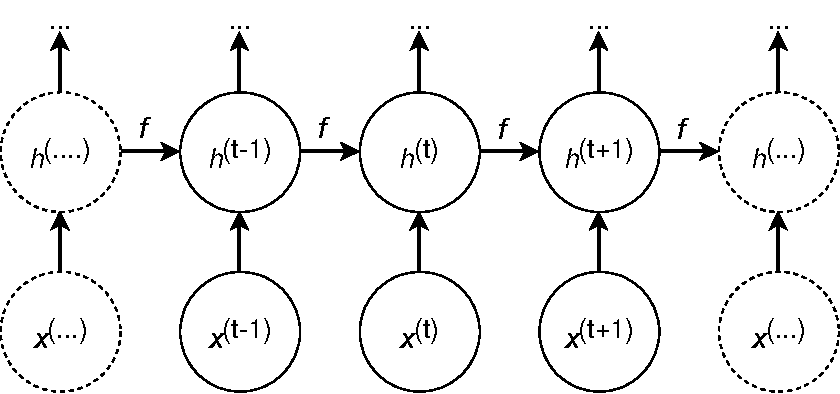
\includegraphics[width=0.8\textwidth]{graphics/rnn-2}
  \caption{An illustration of an RNN for input sequence $x$, where $h$ is the hidden unit activation functions and $f$ a function describing the relationship between two concurrent states~\cite{goodfellow2016deep}.}\label{fig:rnn}
\end{figure}
An illustration of an RNN can be seen in Figure~\ref{fig:rnn} which
shows the context-preserving connections between the hidden nodes
$h^{(t)}$. There are many ways to structure RNNs depending on the
problem at hand, but other structures are out of scope for this project.

Training of RNNs is done using the \textit{backpropagation} algorithm, which is an efficient way to perform gradient descent optimisation of the networks weights. However, in the case of long-term dependencies the gradients tend to become vanishingly small (or in some rare cases tend towards infinity) which hinders training. One solution to this problem is to use so called \textit{gated RNNs}; in particular Long Short-Term Memory Networks (LSTMs).

\subsection{Long Short-Term Memory Networks}
LSTMs are RNNs with a more complicated cell structure for the hidden units, which have shown to much better capture long-term dependencies than the simpler structure of standard hidden units~\cite{hochreiter1997long}. They work by containing an internal state which is regulated by the input.

\begin{figure}[H]
  \centering
  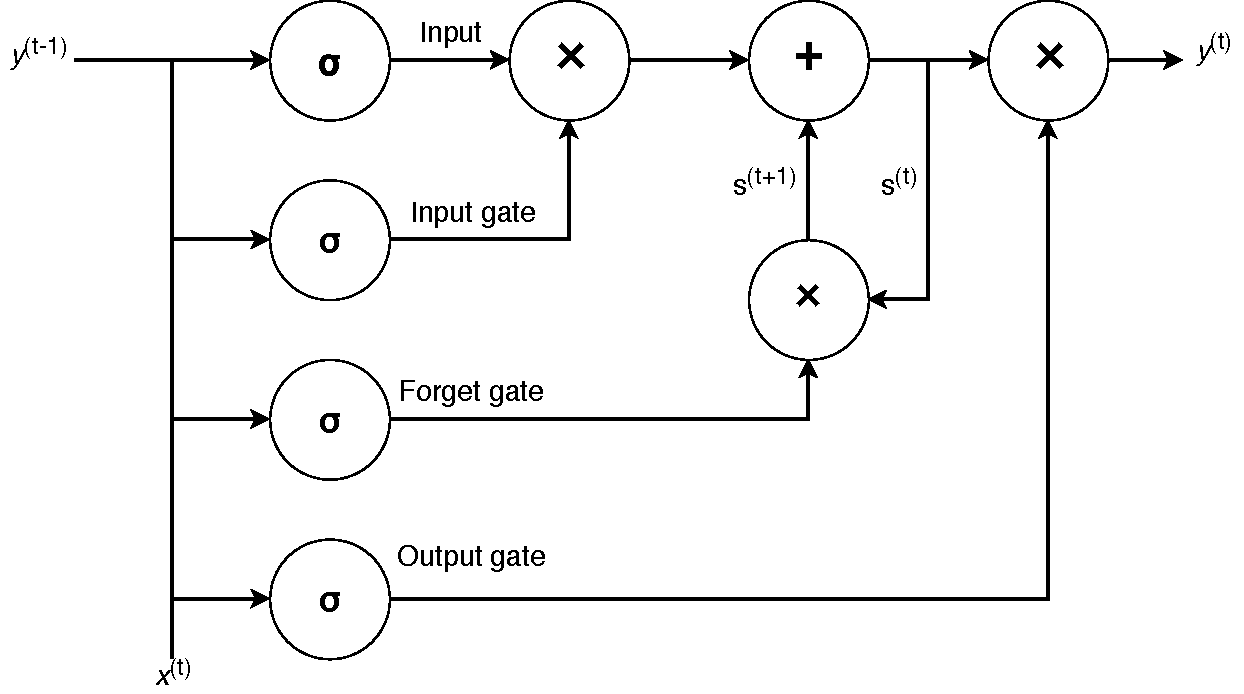
\includegraphics[width=0.8\textwidth]{graphics/lstm-cell}
  \caption{An illustration of an LSTM cell where $x$ is input, $y$ output and $s$ cell state for a specific time point. $\sigma$ indicates a linear combination of inputs passed through the sigmoid function. }\label{fig:lstm-cell}
\end{figure}
As can be seen in Figure~\ref{fig:lstm-cell} an LSTM propagates both the previous output $y^{(t-1)}$ and the previous state $s^{(t-1)}$ to the next cell. This comes at the cost of several more weights that need to be optimised during training, but is a key component for their performance. 
\chapter{Data}
The data was provided by a competition on the website Kaggle for
identifying various types of comments~\cite{toxic-kaggle}. It contains
Wikipedia comments in plain text together with labels indicating toxic
behaviour.

\begin{table}[H]
  \centering
  \caption{Example comments with their labels.}    
  \label{tbl:comments}
  \resizebox{12cm}{!}{%
\begin{tabular}{l|ccccccc}
comment text &  toxic &  severe toxic &  obscene &  threat &  insult
  &  identity hate \\
  \hline
  "\textbackslash n Sure, but the lead must briefly summarize ... &      0 &             0 &        0 &       0 &       0 &              0 \\
TFD \textbackslash n\textbackslash nI think we just eced. I think we respo... &      0 &             0 &        0 &       0 &       0 &              0 \\
 You are gay or antisemmitian? \textbackslash n\textbackslash nArchangel WH... &      1 &             0 &        1 &       0 &       1 &              1 \\
           FUCK YOUR FILTHY MOTHER IN THE ASS, DRY! &      1 &             0 &        1 &       0 &       1 &              0 \\
  I'm Sorry \textbackslash n\textbackslash nI'm sorry I screwed around with ... &      1 &             0 &        0 &       0 &       0 &              0 \\
  I don't believe the Lisak criticism present th... &      0 &             0 &        0 &       0 &       0 &              0 \\
  You had a point, and it's now ammended with ap... &      0 &             0 &        0 &       0 &       0 &              0 \\
  In other words, you're too lazy to actually po... &      0 &             0 &        0 &       0 &       0 &              0 \\
  "\textbackslash nAs for your claims of ""stalking"", that is... &      0 &             0 &        0 &       0 &       0 &              0 \\
  "::::Jmabel; in regards to predominant scholar... &      0 &             0 &        0 &       0 &       0 &              0 \\
\end{tabular}
  }
\end{table}
The different labels of the comments were ``toxic'', ``severe toxic'' ,
``obscene'', ``threat'', ``insult'', and ``identity hate''. Some
truncated comments and their labels can be seen in
Table~\ref{tbl:comments}. 
\begin{figure}[H]
  \centering
  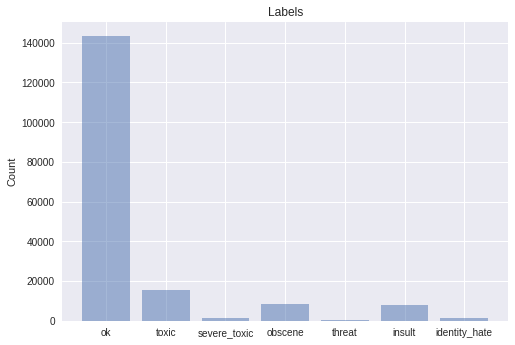
\includegraphics[width=0.8\textwidth]{graphics/label-dist}
  \caption{The count of different labels. Since labels are independent,
    one comment can contribute to several label counts.}\label{fig:labels-dist}
\end{figure}
The data was skewed towards unflagged comments. Figure~\ref{fig:labels-dist} show the counts of the
different labels, where it can be seen that the labels ``severe
toxic'', ``threat'' and ``identity hate'' are increadibly uncommon,
for instance.
\begin{figure}[H]
  \centering
  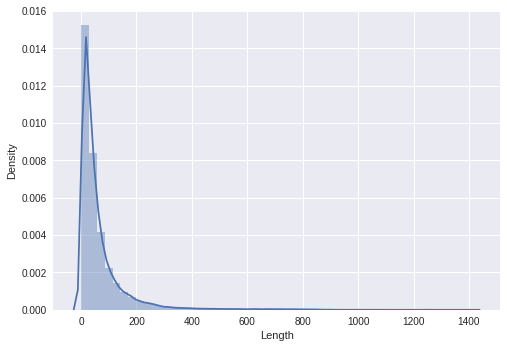
\includegraphics[width=0.8\textwidth]{graphics/comment-word-count}
  \caption{Density plot of comment word counts.}\label{fig:comment-word-count}
\end{figure}
Plotting the word count of the comments show that almost all comments
have less than 200 words in them.	
\chapter{Method}
This chapter describes the data pre-processing and the implementation
process. The implementation goal was to create functional
implementation of an LSTM network using pre-trained FastText embeddings and a
Naive Bayes classifier.

\section{Pre-processing}
The first step was to sanitise the comments using regex
substitution. The pre-trained embeddings 

\section{Naive Bayes Baseline model}
Because 

\section{LSTM Network}

\section{LSTM Network with FastText Embeddings}
To improve the performance of he LSTM model, FastText word embeddings
were investigated. When people from many different countries
communicate online using English, spelling errors are unavoidable.  

naive bayes as baseline

introduce naive LSTM

argue for FastText and online slang

run LSTM with FastText embeddings
	
\chapter{Results}

\begin{table}[H]
  \centering
  \caption{Performance of the Naive Bayes 
    models for the different data labels.}\label{tbl:nb-performance}
 \begin{tabular}{l | r  r | r  r | r  r }
   & \multicolumn{2}{c}{Naive Bayes} & \multicolumn{2}{c}{LSTM} &
                                                                  \multicolumn{2}{c}{LSTM w. FastText} \\
    Label         & Precision & Recall & Precision & Recall & Precision & Recall \\
    \hline 
    Severe toxic  & 0.53 & 0.77 \\
    Obscene       & 0.67 & 0.82 \\
    Threat        & 0.50 & 0.53 \\
    Insult        & 0.65 & 0.79 \\
    Identity hate & 0.54 & 0.67 \\
  \end{tabular}
\end{table}

lstm     0.59, 0.61
fasttext 0.54, 0.67

\begin{tabular}{ |l|l|l| }
  \hline
  \multicolumn{3}{ |c| }{Team sheet} \\
  \hline
  Goalkeeper & GK & Paul Robinson \\ \hline
  \multirow{2}{*}{Naive Bayes} & LB & Lucas Radebe \\
             & DC & Michael Duburry \\
  \multirow{2}{*}{LSTM} & MC & David Batty \\
             & MC & Eirik Bakke \\
  Forward & FW & Jamie McMaster \\ \hline
  \multirow{2}{*}{LSTM w. FastText} & ST & Alan Smith \\
             & ST & Mark Viduka \\
  \hline
\end{tabular}

% \begin{table}[H]
%   \centering
%   \caption{Model MAE \textit{(s)} and MAPE \textit{(\%)} for test trajectories from Bus 3}
%   \label{tbl:models-mae-and-mape-203}
%   \begin{tabular}{l | l | l || l | l | l || l | l | l || l | l | l || l | l | l | }
% %    & \multicolumn{3}{c}{Severe toxic}
% %    & \multicolumn{3}{c}{Obscene}
% %    & \multicolumn{3}{c}{Threat}
% %    & \multicolumn{3}{c}{Insult}
% %    & \multicolumn{3}{c}{Identity hate} \\
%     Naive Bayes
%     \hline \\
%      & 14.9 & 14.9 & 14.9 & 14.9  & 27 & 37 & 56 & 119 \\
%     NN - M1        & 14.79& 14.8& 14.79& 14.79& 30& 41& 61& 123 \\
%     NN - M2        & 10.34& 6.78& 6.77& 1.96& 13& 12& 14& \textbf{11} \\
%     NN - M3       & 10.26& 6.41& 6.68& 2.05& 13& 11& 14& \textbf{11}\\
%     NN - M4        & 10.91& 5.8& 5.77& 1.84& 13& 10& 12& \textbf{11} \\
%     NN - M1 compr.       & 12.02& 12.02& 12.02& 12.02& 35& 47& 71& 145 \\
%     NN - M2 compr.       & 3.81& 3.49& 2.58& \textbf{1.57}& \textbf{8}& \textbf{9}& \textbf{11}& 15 \\
%     NN - M3 compr.       & \textbf{3.66}& \textbf{3.19}& \textbf{2.38}& 1.67& \textbf{8}& \textbf{9}& \textbf{11}& 16 \\
%     NN - M4 compr.       & 3.67& 3.6& 2.62& 1.69& \textbf{8} & 10& 13& 18 \\
%     GPR        &  12.17 & 10.72 & 10.75 & 13.42 & 26 &  34 & 61 &  155  \\
%   \end{tabular}
% \end{table} 
\chapter{Discussion}
This chapter discusses the validity of the results and critically
evaluates the method used.

%['year’s', 'funnyask', 'aolisms', 'hurlburt', '5-20%', 'εκκλησίας', 'cause:', 'máltilfinningu.', 'magneto-motive', '120.148.90.195', 'circumcising;', 'enough...not', 'sanhedrin.', 'edisons', 'two-parter...', '10g;', 'sarcasm==', 'wikipedia:make_technical_articles_accessible', 'multics.', 'speidels', 'link==', 'thacker', 'concerned:', 'adkeeyey', 'sdgbfhyufjfsjckfsijldxhltgfgn', 'http://www.officialcharts.com/', 'favre.', 'edittor.', 'shouries', 'htet', 'btw...', 'florentino', 'istanbul.3', 'agada', 'distinct...', 'ss=wikitable', 'periods/sentences.', 'bandelier', 'armeniens', '18:14', 'dictators.', 'iceage', 'team’s', '==ruler==', 'වාසභුමිය', 'user:thedeletator', 'wp:npov:as', 'توانیم', 'spam/commerical', '.आपल्या']

\section{Data pre-processing}
The pre-processing step leaves a lot of room for improvement. A much
more thorough investigation of the data and the pre-trained embeddings
should have been performed to find more relevant rules for
sanitisation and stop words. 

\subsection{The large number of null embeddings}
The number of null embeddings was 47\%, which means that around half
of the training data was practically useless. Needless to say, that is
a terrible result. Investigating the
problematic words show a mix of nonsense, spelling errors, non-English
words, and web addresses, but also several words that could have been found if sanitisation was
done more rigorously. Example of these words are ``year’s'' and
``cause:'', which would have been a non-issue if accents and colons
were sanitised. There might also be several undiscovered cases where a proper
word is simply represented on a different form in the pre-trained
embeddings than in the vocabulary, such as there not being an embedding for the word
``that's'', but one for ``thats''.

\section{Model performances}
The baseline Naive Bayes performed admirably, and while its precision was quite a
bit worse than the LSTM models, it had the best recall of all
models. However, the LSTM models were only trained for 3 epochs
because of time constrains, and no parameter optimisation was
performed. So while the Naive Bayes model is as good as it gets, the
LSTM models most certainly have a lot of room for improvement, such as
training with early stopping, and using grid search to optimise hyper-parameters.

Another aspect to consider is the amount of data required to train a
model. A Neural Network requires much more data than a Naive Bayes
model to reach adequate performance, and so in situations with lower
data volumes, Naive Bayes is hypothesised to outperform the LSTM
models. It would be interesting to evaluate model performance for
different data volumes, but such an investigation has been discarded
because of time constraints. 

In light of this discussion, performance of the LSTM models should be
seen as a baseline, with lots of areas of improvement. 
\chapter{Conslusion}
o hai
 
\cleardoublepage

% --------------------------
% Back matter
% --------------------------
{%
\setstretch{1.1}
\renewcommand{\bibfont}{\normalfont\small}
\setlength{\biblabelsep}{0pt}
\setlength{\bibitemsep}{0.5\baselineskip plus 0.5\baselineskip}
\printbibliography[nottype=online]
\printbibliography[heading=subbibliography,title={Webseiten},type=online,prefixnumbers={@}]
}
\cleardoublepage

%\cleardoublepage

%\cleardoublepage

%\input{content/colophon}
%\cleardoublepage

%\input{content/declaration}
\clearpage
\newpage
\mbox{}

% **************************************************
% End of Document CONTENT
% **************************************************
\end{document}
